\section{Equazione semiclassica di Boltzmann}
Nello studio di una qualsiasi nanostruttura, è necessario mettere a contatto questa struttura con i dispositivi di misura macroscopici. Tipicamente, ciò viene fatto strutturando elettrodi molto più grandi dei sistemi studiati e mettendoli in contatto con questi ultimi. Un tale elettrodo funge da serbatoio ideale (sia termico che di particelle) per gli elettroni. Consideriamo quindi un sistema mesoscopico\mn{Per mesoscopico si intende un sistema di dimensioni intermedie tra quelle microscopiche e quelle macroscopiche. Possiamo quindi dire più semplicemente che tale sistema ha dimensioni piccole.} composto da un conduttore (ad esempio un metallo, un semiconduttore o un isolante topologico) in contatto con due serbatoi $L$ ed $R$, di dimensioni macroscopiche che possono fornire sia cariche (più precisamente elettroni) che energia, come in figura:
\begin{figure}[H]
   \centering
    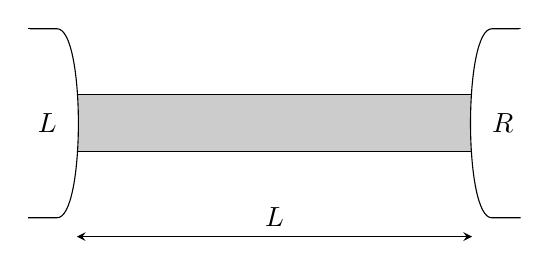
\begin{tikzpicture}[scale=1.2]
        %sistema mesoscopico
        \draw[fill=gray!40!] (-2.11,0.3) -- (2.11,0.3) -- (2.11,-0.3) -- (-2.11,-0.3) -- cycle;
        %Reservoir
        \draw[fill=white] (-2.6,-1) -- (-2.3,-1) .. controls (-2,-1) and (-2,1) .. (-2.3,1) -- (-2.6,1) -- cycle;
        \draw[white,thick,shorten <= 0.22pt,shorten >= 0.22pt] (-2.6,-1) -- (-2.6,1);
        \draw[fill=white] (2.6,-1) -- (2.3,-1) .. controls (2,-1) and (2,1) .. (2.3,1) -- (2.6,1) -- cycle;
        \draw[white,thick,shorten <= 0.22pt,shorten >= 0.22pt] (2.6,-1) -- (2.6,1);
        % Etichette nei contatti
        \node[left] at (-2.2,0) {$L$};
        \node[right] at (2.2,0) {$R$};
        % Distanza L con frecce
        \draw[stealth-stealth,shorten <= -0.11cm, shorten >= -0.11cm] (-2,-1.2) -- (2,-1.2) node[midway, above] {$L$};
    \end{tikzpicture}
\end{figure}
\hspace{-0.6cm}Per serbatoio ideale intendiamo che il numero di elettroni al suo interno è talmente elevato che la sua temperatura e il suo potenziale chimico restano invariati anche se un elettrone abbandona o entra nel reservoir, in quanto $N\approx N+1$ per $N$ grande.\\
Tale assunzione implica che quando il numero di elettroni del reservoir varia, questo ritorni istantaneamente ad uno stato di equilibrio, rendendo possibile descrivere gli elettroni dei reservoir mediante la distribuzione di Fermi-Dirac:
\begin{equation}
    f_D(E,\mu,T)
    = \frac{1}{\exp \bigl[ (E - \mu)/(k_B T) \bigr] + 1}
    \label{eq:distribuzione_Fermi-Dirac}
\end{equation}
Essa rappresenta il numero medio di elettroni ad energia $E$, fissata la temperatura $T$ e potenziale chimico $\mu$.\\
Ricordiamo che tale distribuzione segue l'andamento riportato in figura:
\begin{figure}[H]
    \centering
    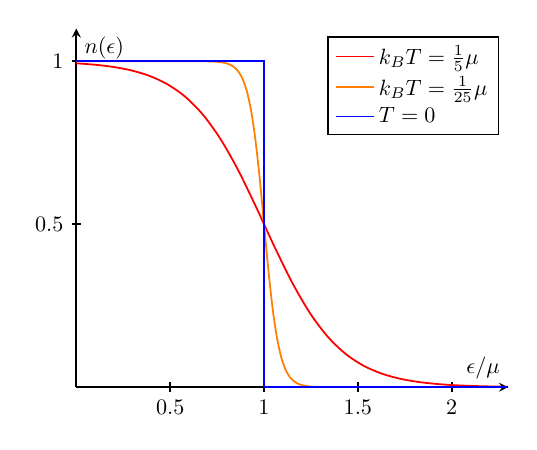
\begin{tikzpicture}[scale=.8]
        \begin{axis}[
            xlabel=$\epsilon/\mu$,
            ylabel=$n(\epsilon)$,
            domain=0:2.3,ymax=1.1,
            ytick={0.5,1},
            smooth,thick,
            axis lines=center,
            every tick/.style={thick},
            legend cell align=left]
      
          % Graphs
          \def\chempot{1}
          \def\n#1{1/(e^(#1*(x - \chempot)) + 1)}
          \addplot[color=red]{\n{5}};
          \addplot[color=orange,samples=100]{\n{25}};
          \addplot[const plot,color=blue] coordinates {(0,1) (\chempot,0) (2.3,0)};
      
          \legend{$k_\text{B} T = \frac{1}{5} \mu$,$k_\text{B} T = \frac{1}{25} \mu$,$T = 0$}.
        \end{axis}
      \end{tikzpicture}
\end{figure}
\textbf{DISEGNO PROVVISORIO}\\
Quando $T\to 0$, essa tende a una funzione a gradino, mentre a temperatura finita ha un andamento più smussato.\\
In generale, i due serbatoi possono avere temperature $T_L$ e $T_R$ o potenziali chimici $\mu_L$ e $\mu_R$ diversi. Il modo più semplice per avere, ad esempio, due potenziali chimici diversi è quello di applicare una differenza di potenziale tra i due serbatoi\mn{Se invece volessimo realizzare una differenza di temperatura è sufficiente applicare un gradiente termico.} collegandoli ad un generatore di tensione, il quale permetterà di modulare $\mu_L$ e $\mu_R$:
\begin{figure}[H]
    \centering
     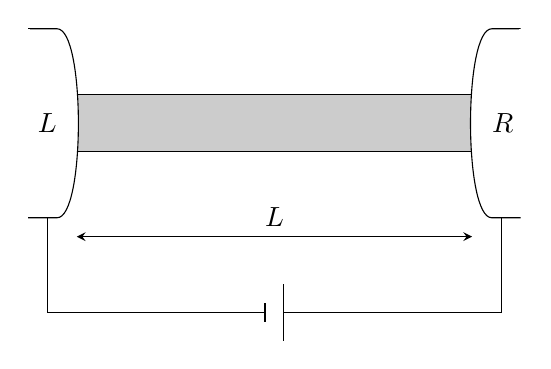
\begin{tikzpicture}[scale=1.2]
        %sistema mesoscopico
        \draw[fill=gray!40!] (-2.11,0.3) -- (2.11,0.3) -- (2.11,-0.3) -- (-2.11,-0.3) -- cycle;
        %Reservoir
        \draw[fill=white] (-2.6,-1) -- (-2.3,-1) .. controls (-2,-1) and (-2,1) .. (-2.3,1) -- (-2.6,1) -- cycle;
        \draw[white,thick,shorten <= 0.22pt,shorten >= 0.22pt] (-2.6,-1) -- (-2.6,1);
        \draw[fill=white] (2.6,-1) -- (2.3,-1) .. controls (2,-1) and (2,1) .. (2.3,1) -- (2.6,1) -- cycle;
        \draw[white,thick,shorten <= 0.22pt,shorten >= 0.22pt] (2.6,-1) -- (2.6,1);
        % Etichette nei contatti
        \node[left] at (-2.2,0) {$L$};
        \node[right] at (2.2,0) {$R$};
        % Distanza L con frecce
        \draw[stealth-stealth,shorten <= -0.11cm, shorten >= -0.11cm] (-2,-1.2) -- (2,-1.2) node[midway, above] {$L$};
        % circuito
        \draw (-2.4,-1) -- (-2.4,-2) -- (-0.1,-2);
        \draw[thick] (-0.1,-2.1) -- (-0.1,-1.9);
        \draw (0.1,-2.3) -- (0.1,-1.7);
        \draw (0.1,-2) -- (2.4,-2) -- (2.4,-1);
    \end{tikzpicture}
 \end{figure}
\hspace{-0.6cm}In conseguenza a tale differenza di potenziale chimico, si verificherà un flusso di elettroni tra i due reservoir, facendo comunque restare questi ultimi in equilibrio per le precedenti assunzioni.\\
(Di questo paragrafetto lascerei solo la prima nota, forse mettendola nella discussione sopra sui serbatoi ideali)Supponiamo che nei due serbatoi il sistema elettronico rimanga in equilibrio anche in presenza di una caduta di tensione o di una differenza di temperatura e, se vi è un flusso di corrente, assumiamo che nei due serbatoi avvenga un rilassamento istantaneo degli elettroni\sn{Per rilassamento istantaneo si intende un processo in cui un sistema passa da uno stato di non equilibrio a uno stato di equilibrio in un tempo trascurabilmente breve, praticamente istantaneo rispetto alle scale temporali del fenomeno in esame.}, i quali rimangono in equilibrio. Ciò significa che gli elettroni nei serbatoi possono essere sempre descritti dalla distribuzione di Fermi-Dirac, la quale rimane invariata\sn{Dubbio mio: ma visto che applichiamo il voltage drop non cambia il potenziale chimico? e quindi la distribuzione di Fermi-Dirac? probabilmente intende che la funzione di distribuzione è sempre una FD, come forma funzionale, ad un opportuno $\mu$}.\\
Studiamo il problema con una teoria semiclassica, dove con tale espressione intendiamo che nell'equazione che descrive il sistema figurano sia termini di tipo classico che altri di tipo quantistico. Più precisamente, descriviamo gli elettroni come particelle classiche e riteniamo la loro posizione e il loro impulso conoscibili contemporaneamente con precisione sufficientemente grande, figurando questi come variabili classiche in alcuni termini, mentre convenientemente come operatori quantistici in altri. Quantitativamente, ciò è ragionevole quando la lunghezza d'onda di Fermi, che rappresenta la larghezza del pacchetto d'onda e quindi l'incertezza sulla posizione della particella data dal principio di indeterminazione di Heisenberg, data da
\begin{equation*}
    \lambda_F=\frac{2\pi}{k_F}=\frac{2\pi\hbar}{\sqrt{2mE_F}},
\end{equation*}
essendo $E_F$ l'energia di Fermi e $m$ la massa efficace dell'elettrone, è molto più piccola di tutte le scale di lunghezza del sistema. Ciò significa che $\lambda_F$ deve essere molto più piccola delle dimensioni tipiche del sistema e dei diversi liberi cammini medi, cioè delle distanze percorse mediamente da un elettrone tra due eventi consecutivi di scattering della medesima tipologia. In particolare, nella nostra trattazione siamo interessati a tre tipi di liberi cammini medi:
\begin{itemize}[leftmargin=0.5cm]
    \item la lunghezza di scattering elastico $\ell_{\rm el}$, associata allo scattering degli elettroni con le impurità del sistema;
    \item la lunghezza di scattering elettrone-elettrone $\ell_{\rm e,e}$, legata allo scattering di elettroni con altri elettroni e dunque dovuta all'interazione coulombiana;
    \item la lunghezza di scattering elettrone-fonone $\ell_{\rm e,ph}$, associata allo scattering degli elettroni con i fononi del sistema.
\end{itemize}
Precisiamo i seguenti fatti:
\begin{itemize}[leftmargin=0.5cm]
    \item lo scattering tra elettroni e impurità è elastico, per cui l'energia dell'elettrone si conserva;
    \item lo scattering elettrone-elettrone non conserva l'energia del singolo elettrone ma l'energia totale dei due elettroni. Ciò è dovuto al fatto che nello scattering i due elettroni possono scambiare energia, come possiamo vedere nel seguente diagramma:
    \begin{figure}[H]
        \centering
        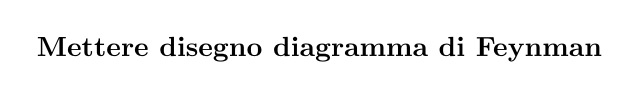
\begin{tikzpicture}
            \node at (0,0) {\textbf{Mettere disegno diagramma di Feynman}};
        \end{tikzpicture}
    \end{figure}
    Per quanto detto avremo che, se $E_1$ ed $E_2$ sono le energie prima dello scattering e $E_1'$ ed $E_2'$ le energie dopo lo scattering, allora avremo che in generale $E_1 \neq E_1'$ e $E_2 \neq E_2'$ ma $E_1 + E_2 = E_1' + E_2'$;
    \item nello scattering elettrone-fonone, in cui si ha l'assorbimento o l'emissione di un fonone di energia $\hbar \omega$, l'energia non si conserva, in quanto dopo lo scattering l'elettrone inizialmente avente energia $E$ avrà energia $E \pm \hbar \omega$, come possiamo vedere nei seguenti diagrammi:
    \begin{figure}[H]
        \centering
        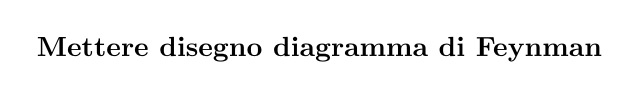
\begin{tikzpicture}
            \node at (0,0) {\textbf{Mettere disegno diagramma di Feynman}};
        \end{tikzpicture}
    \end{figure}
\end{itemize}
Un ulteriore precisione va fatta riguardo all'efficienza dei processi di scattering. Infatti, esiste un'ulteriore lunghezza caratteristica chiamata lunghezza di coerenza $\ell_\phi=v\tau_\phi$, dove $v$ è la velocità di gruppo e $\tau_\phi$ è il tempo che intercorre tra due processi di scattering a seguito dei quali viene modificata la fase della funzione d'onda della particella. Se $\ell_\phi$ è piccolo, cioè $\tau_\phi$ è piccolo, diciamo che lo scattering è efficiente e si ha il cosiddetto fenomeno di "dephasing", ossia una randomizzazione della fase della funzione d'onda. In conseguenza a ciò vengono meno tutti i processi coerenti, come i processi di interferenza. Nel momento in cui vengono meno questi ultimi, la particella, a meno di correzioni di cui terremo conto, si comporta come una particella classica. Questo tipo di descrizione è tipico della fisica dei semiconduttori, ma bisogna prestare attenzione al tipo di processo che si sta studiando: ad esempio, tale approccio non funziona per studiare l'assorbimento inter-banda in cui vogliamo studiare il passaggio di un elettrone dalla banda di valenza alla banda di conduzione, in quanto il concetto di banda non esiste classicamente; al contrario, tale approccio funziona quando studiamo trasporto in corrente continua o modulato debolmente.\\
Ritornando al nostro sistema mesoscopico collegato ai due serbatoi, ci proponiamo di trovare la funzione di distribuzione degli elettroni in tale sistema.\\
Cerchiamo quindi una funzione\sn{Notiamo che la validità del concetto di funzione di distribuzione $f(\vb{r}, \vb{p},t)$ poggia sull'assunzione fatta precedentemente su $\lambda_F$ e $\ell_\phi$.} $f(\vb{r},\vb{p},t)$ tale che la quantità
\begin{equation*}
    f(\vb{r},\vb{p},t) \frac{\dd[3]{\vb{r}} \dd[3]{\vb{p}}}{(2 \pi \hbar)^3},
\end{equation*}
cioè il prodotto tra essa e il volume elementare dello spazio delle fasi, ci dia il numero di elettroni aventi posizione tra $\vb{r}$ e $\dd[3]{\vb{r}}$ e impulso tra $\vb{p}$ e $\dd[3]{\vb{p}}$. In particolare vale la seguente condizioni di normalizzazione:
\begin{equation}
    \int g_S\frac{\dd[3]{\vb{r}}\dd[3]{\vb{p}}}{(2\pi \hbar)^3} f(\vb{r},\vb{p},t) = N,
\end{equation}
dove $N$ è il numero totale di elettroni del nostro sistema mesoscopico e $g_s$ è la degenerazione di spin, che nel caso in esame è semplicemente pari a 2.\\
Per trovare la funzione di distribuzione ne studiamo l'evoluzione temporale. Dopo un tempo $\dd{t}$, la funzione di distribuzione sarà $f(\vb{r} + \vb{v} \dd{t}, \vb{p} + \vb{F} \dd{t}, t + \dd{t})$, dove $\vb{v}$ è la velocità dell'elettrone e $\vb{F}$ è la forza che agisce su di esso, generata dal campo elettromagnetico dovuto alla caduta di potenziale
%che assumiamo una dipendenza spaziale regolare
. Se non avvengono fenomeni di scattering, per il teorema di Liouville\mn{Esso afferma che un volumetto $\dd[3]\vb{r}\dd[3]\vb{p}$ dello spazio delle fasi centrato in $(\vb{r},\vb{p})$ evolve nello spazio delle fasi rimanendo invariato.(da sistemare)} la funzione di distribuzione rimane costante, ossia
\begin{equation*}
    f(\vb{r} + \vb{v} \dd{t}, \vb{p} + \vb{F} \dd{t}, t + \dd{t}) - f(\vb{r}, \vb{p}, t)
    =0
\end{equation*}
Se invece avvengono fenomeni di scattering, la funzione di distribuzione varia. Denotata con $I_{\rm coll}[f] \dd{t}$ tale differenza, dove $I_{\rm coll}[f]$ è detto integrale collisionale e tiene conto di tutti i processi di scattering, abbiamo che
\begin{equation}
    f(\vb{r} + \vb{v} \dd{t}, \vb{p} + \vb{F} \dd{t}, t + \dd{t}) - f(\vb{r}, \vb{p}, t)
    =I_{\rm coll}[f] \dd{t}
    \label{eq:differenza_funzione_distribuzione_con_collisioni}
\end{equation}
Il membro destro dell'Equazione \eqref{eq:differenza_funzione_distribuzione_con_collisioni} rappresenta il termine quantistico nell'equazione che descrive il nostro sistema.\\
Consideriamo il membro di sinistra ed espandiamo al primo in ordine in $\dd{t}$, ottenendo
\begin{equation*}
    \begin{split}
        & \hspace{0.1cm} f(\vb{r} + \vb{v} \dd{t}, \vb{p} + \vb{F} \dd{t}, t + \dd{t}) - f(\vb{r}, \vb{p}, t)
        \\
        = & \hspace{0.1cm} f(\vb{r}, \vb{p}, t) + \pdv{f}{\vb{r}} \vdot \vb{v} \dd{t} + \pdv{f}{\vb{p}} \vdot \vb{F} \dd{t} + \pdv{f}{t} \dd{t} - f(\vb{r}, \vb{p}, t) + \smallO{(\dd{t})^2}
        \\
        \approx & \hspace{0.1cm} \pdv{f}{\vb{r}} \vdot \vb{v} \dd{t} + \pdv{f}{\vb{p}} \vdot \vb{F} \dd{t} + \pdv{f}{t} \dd{t}
    \end{split}
\end{equation*}
Utilizzando quanto trovato, otteniamo
\begin{equation}
    \pdv{f}{\vb{r}} \vdot \vb{v} + \pdv{f}{\vb{p}} \vdot \vb{F} + \pdv{f}{t}
    =I_{\rm coll}[f],
    \label{eq:equazione_di_Boltzmann}
\end{equation}
che è chiamata equazione di Boltzmann.\\
Puntualizziamo che in assenza del termine collisionale, l'equazione di Boltzmann prende il nome di equazione di Vlasov:
\begin{equation}
    \pdv{f}{\vb{r}} \vdot \vb{v} + \pdv{f}{\vb{p}} \vdot \vb{F} + \pdv{f}{t}
    =0.
    \label{eq:equazione_di_Vlasov}
\end{equation}
Osserviamo che tale equazione è applicabile in poche situazioni, in quanto abbiamo supposto che i processi di scattering siano trascurabili ma allo stesso tempo che avvenga il fenomeno di dephasing.\\
Torniamo adesso all'\eqref{eq:equazione_di_Boltzmann}. E' utile esprimere la dipendenza da $\vb{p}$ tramite le coordinate sferiche, dunque dividendo la dipendenza dalla parte angolare da quella radiale. In tali termini, la funzione di distribuzione sarà nella forma $f(\vb{r},\vu{p},E)$, dove abbiamo messo l'energia al posto del modulo $p$ perché la relazione di dispersione è del tipo
\begin{equation*}
    \varepsilon(\vb{p})=
    \frac{\vb{p}^2}{2m}
\end{equation*}
dove $m$ è la massa efficace dell'elettrone\mn{Infatti stiamo usando implicitamente l'approssimazione di elettroni liberi.}.\\
In tale forma, il termine contenente la derivata rispetto a $\vb{p}$ nell'\eqrefcustom{eq:equazione_di_Boltzmann} diventa
\begin{equation*}
    \pdv{f}{\vb{p}} \vdot \vb{F}
    =\pdv{f}{\vu{p}} \pdv{\vu{p}}{\vb{p}} \vdot \vb{F} + \pdv{f}{E} \pdv{E}{\vb{p}}\vdot \vb{F} 
\end{equation*}
Tuttavia, il primo termine del membro di destra risulta essere trascurabile, vedremo a breve perché.\\
Possiamo quindi scrivere
\begin{equation*}
    \pdv{f}{\vb{p}} \vdot \vb{F}
    =\pdv{f}{E} \pdv{E}{\vb{p}}\vdot \vb{F}
\end{equation*}
D'altra parte, il gradiente della relazione di dispersione rispetto all'impulso $\vb{p}$ non è altro che la velocità di gruppo $\vb{v}$,\mn{Infatti, esplicitamente si ha
\begin{equation*}
    \grad_{\vb{p}} \varepsilon(\vb{p})
    =\grad_{\vb{p}} \frac{\vb{p}^2}{2m}
    =\frac{\vb{p}}{m}
    \equiv \vb{v}
\end{equation*}} per cui in definitiva abbiamo che
\begin{equation*}
    \pdv{f}{\vb{p}} \vdot \vb{F}
    =\pdv{f}{E} \vb{v} \vdot \vb{F}
\end{equation*}
Supponiamo adesso che la forza sia dovuta soltanto al campo elettrico, dunque sia nella forma $\vb{F}=q\vb{E}$ dove $q$ è la carica. Allora, ricordando che $\vb{E}=-\partial_{\vb{r}} \phi$, per quanto detto il termine dell'\eqref{eq:equazione_di_Boltzmann} contenente $\vb{F}$ diventa
\begin{equation*}
    \pdv{f}{\vb{p}} \vdot \vb{F}
    =\pdv{f}{E} \vb{v} \vdot \qty( -q \pdv{\phi}{\vb{r}} )
    =\pdv{f}{E} \qty( -q \pdv{\phi}{\vb{r}} ) \vdot \vb{v}
\end{equation*}
e dunque possiamo riscrivere l'\eqrefcustom{eq:equazione_di_Boltzmann} come
\begin{equation*}
    \pdv{f}{\vb{r}} \vdot \vb{v} + \pdv{f}{E} \qty( -q \pdv{\phi}{\vb{r}} ) \vdot \vb{v} + \pdv{f}{t}
    =I_{\rm coll}[f]
\end{equation*}
ovvero, raggruppando i termini,
\begin{equation}
    \qty( \pdv{f}{\vb{r}} - q \pdv{\phi}{\vb{r}} \pdv{f}{E} ) \vdot \vb{v} + \pdv{f}{t}
    =I_{\rm coll}[f]
    \label{eq:equazione_di_Boltzmann_con_campo}
\end{equation}
Se inglobiamo nell'energia la dipendenza del potenziale dalla posizione, il che corrisponde a dire che $f$ ha una dipendenza del tipo $f(\vb{r},\vb{p}, E - q \phi(\vb{r}))$, il termine tra parentesi della \eqref{eq:equazione_di_Boltzmann_con_campo} diventa proprio $\pdv*{f}{\vb{r}}$, per cui possiamo scrivere più sinteticamente
\begin{equation}
    \pdv{f}{\vb{r}} \vdot \vb{v} + \pdv{f}{t}
    =I_{\rm coll}[f]
    \label{eq:equazione_di_Boltzmann_con_campo_sintetica}
\end{equation}
Osserviamo che se $f(\vb{r},\vb{p}, E - q \phi(\vb{r}))$ si comportasse come una funzione di distribuzione di Fermi-Dirac, ciò significherebbe che nell'\eqrefcustom{eq:distribuzione_Fermi-Dirac} al posto di $\mu$ dovremmo scrivere $\mu + q\phi(\vb{r})$, cioè è come se ci ritrovassimo un potenziale chimico che dipende dalla posizione. Come vedremo, quando $f$ prende la forma di una funziona di Fermi-Dirac efficace, tale $\mu$ prenderà il nome di potenziale elettrochimico.\\
Prima di proseguire, facciamo una stima dell'ordine del termine relativo alla derivata rispetto a $\vu{p}$ che abbiamo trascurato, in modo da capire quanto è grande l'errore che commettiamo nel trascurarlo. Osserviamo che $\pdv*{f}{\vu{p}}$ è adimensionale perché $f$ è una densità di probabilità, dunque possiamo concentrarci sulla parte $\pdv*{\vu{p}}{\vb{p}} \vdot \vb{F}$: nella parte $\pdv*{\vu{p}}{\vb{p}}$, $\vu{p}$ non ha dimensioni, mentre $\vb{p}$ ha le dimensioni di un impulso ed in particolare è dell'ordine dell'impulso di Fermi $p_F$; $F$ invece è una forza elettrica che è dell'ordine della carica moltiplicata per la differenza di tensione applicata divisa la lunghezza del campione. In definitiva abbiamo:
\begin{equation*}
    \qty[ \pdv{f}{\vu{p}} \pdv{\vu{p}}{\vb{p}} \vdot \vb{F} ]
    \sim \frac{1}{p_F} \frac{qV}{L}
\end{equation*}
Moltiplicando e dividendo per $\frac{p_F}{m}$ otteniamo
\begin{equation*}
    \frac{1}{p_F} \frac{qV}{L}
    =\frac{1}{p_F} \frac{qV}{L} \frac{p_F}{m} \frac{m}{p_F}
    =qV \frac{m}{p_F^2} \frac{1}{L} \frac{p_F}{m}
\end{equation*}
Notiamo che $m/p_F^2$ è dell'ordine dell'inverso dell'energia di Fermi, ossia $1/E_F$, mentre $p_F/m$ è dell'ordine della velocità di Fermi $v_F$. In definitiva otteniamo
\begin{equation*}
    \frac{1}{p_F} \frac{qV}{L}
    \sim \frac{qV}{E_F} \frac{v_F}{L}
\end{equation*}
Il termine $v_F/L$ rappresenta la scala dell'inverso dei tempi tipici dell'\eqrefcustom{eq:equazione_di_Boltzmann_con_campo_sintetica}, dunque per capire se tale termine è trascurabile dobbiamo guardare l'ordine di grandezza di $qV/E_F$. In un conduttore, l'energia di Fermi è tipicamente dell'ordine dell'eV o di frazioni dell'eV, mentre $qV$ in genere è dell'ordine dei $\rm \mu eV$, dunque tale termine risulta essere dell'ordine di $10^{-6}$, per cui è lecito trascurarlo. Precisiamo che omettere tale termine equivale sostanzialmente a trascurare il disturbo nella parte angolare della funzione di distribuzione dovuto a una tensione o ad un gradiente termico.
\begin{example}[Equazione di Boltzmann per un filo ballistico.]
    Consideriamo un filo quasi-unidimensionale come quello riportato nella figura seguente:\mn{Disegno da fare il Latex, ora mi secco.}
    \begin{figure}[H]
        \centering
        \includegraphics[width=0.7\textwidth]{Immagini/Ballistic_wire.png}
    \end{figure}
    Diciamo che tale sistema è quasi-unidimensionale perché supponiamo che l'ampiezza $W$ del filo sia molto minore della lunghezza $L$ del filo stesso.\\
    Supponiamo che non contenga impurità, sia perfettamente rettangolare e abbia bordi regolari, in modo che risulti $I_{\rm coll}[f]=0$. Nel limite statico, in cui $\partial_t f=0$, l'\eqrefcustom{eq:equazione_di_Boltzmann} assumerà allora forma
    \begin{equation*}
        \vb{v} \vdot \grad_{\vb{r}} f(\vb{r},\vu{p},E)
        =0
    \end{equation*}
    Supponendo che i serbatoi sinistro e destro seguano rispettivamente dele distribuzioni di Fermi-Dirac $f_L(E)$ ed $f_R(E)$, la funzione di distribuzione sarà data da:
    \begin{equation*}
        f(\vb{r},\vu{p},E)
        =
        \begin{cases}
            f_L(E) & \text{se } \vu{p}_x<0 \\
            f_R(E) & \text{se } \vu{p}_x>0
        \end{cases}
    \end{equation*}
    Il risultato trovato ci dice che, in assenza di collisioni, i due serbatoi restano indipendenti; inoltre gli elettroni iniettati da sinistra seguono la funzione di distribuzione del serbatoio sinistro anche nel sistema mesoscopico (cioè dentro il cavo) e gli elettroni iniettati da destra nel sistema avranno la funzione di distribuzione del serbatoio destro.\mn{Così come riportato in \cite{Heikkila}, ciò significa che "Il sistema di elettroni all'interno del filo è quindi composto da elettroni che si muovono verso sinistra e elettroni che si muovono verso destra, che non si mescolano in assenza di diffusione e che sono distribuiti in energia secondo le funzioni di distribuzione nei serbatoi da cui provengono."}
\end{example}
\section{Osservabili}
Il motivo per cui siamo interessati a trovare la funzione di distribuzione è che possiamo esprimere le osservabili del sistema in termini di essa. In particolare, la densità spaziale di portatori di carica del sistema sarà data da
\begin{equation*}
    n(\vb{r})
    =g_s \int \frac{\dd[3]{\vb{p}}}{(2 \pi \hbar)^3} f(\vb{r},\vb{p},t).
\end{equation*}
Risulta immediato verificare che integrando $n(\vb{r})$ in tutto il volume spaziale si ottiene il numero di elettroni del sistema. Analogamente, la densità di corrente sarà data da
\begin{equation*}
    \vb{j}_c(\vb{r})
    =-e g_s \int \frac{\dd[3]{\vb{p}}}{(2 \pi \hbar)^3} \vb{v}(\vb{p}) f(\vb{r},\vb{p}),
\end{equation*}
dove abbiamo scritto la velocità come $\vb{v(p)}$ per sottolineare che essa è data da $\grad_p \varepsilon(\vb{p})$.
Passando in coordinate polari possiamo riscrivere tale quantità come
\begin{equation*}
    \vb{j}_c(\vb{r})
    =-e g_s \int \dd{p} p^2 \int \frac{\dd{\vu{p}}}{(2\pi\hbar)^3} \vb{v}(\vb{p}) f(\vb{r},\vu{p})
\end{equation*}
dove l'integrazione rispetto a $\vu{p}$ è esplicitamente data da
\begin{equation*}
    \int \dd{\vu{p}}
    =\int_{0}^{2\pi} \dd{\varphi} \int_{0}^{\pi} \dd{\vartheta} \sin{\vartheta}
\end{equation*}
Se adesso esprimiamo $p^2$ come $p^2=2mE$, da cui segue che $2p \dd{p}=2m \dd{E}$, abbiamo che
\begin{equation*}
    \dd{p} p^2
    =\sqrt{2} m^{\frac{3}{2}} \sqrt{E} \dd{E}
\end{equation*}
e inoltre possiamo riscrivere $\vb{j}_c$ come
\begin{equation*}
    \vb{j}_c(\vb{r})
    =-e \int \dd{E} N(E) \int \frac{\dd{\vu{p}}}{4\pi} \vb{v}(\vb{p}) f(\vb{r},\vu{p})
\end{equation*}
dove
\begin{equation*}
    N(E)
    =\frac{\sqrt{2E} m^{\frac{3}{2}}}{\pi^2 \hbar^3}
\end{equation*}
è la densità degli stati di una particella libera in un sistema tridimensionale.\\
%che ha una dipendenza dall'energia a radici. Però non si separava la despicità di tendenza angolare, di solito il fatto che l'energia di un tesoro dal modulo si cambiava la gaffa di gaffa. Perché la partangolare è da se mangiata quando fai il genico, questo come comunque non sai qua che succederà, che da dividere in ghiaccio in altri. Se esistisci questo conto in 2D come va a reprendere gli stati, flat, solamente. Se la faccio in 1D come direi le densità degli stati di raggiungere. Quindi in 2D a meno di questo 3D, se li facesti la stessa cosa, immaginando un sistema 2D, la densità degli stati se parte più che lo su 2M viene una costante. Se la faccio invece in 3D, mi viene una roba di questo tipo che è una divergenza integrabile. La differenza della densità registra di le fattore singuramente divano, sono solide. Tutte divergenze integrabili, perché se hai preso un conto e provate una divergenza di un'insidestra che non è integrabile, hai risposto. Perché il flat da c'è, non è possibile che da una cosa in cui contate gli stati viene vengono più, non mi corrisponde una cosa che non è contabile, perché se le partite da una cosa che è integrabile, hai fatto soltanto un cambiamento di variabili per coppare la fittura. Questo è un miscule che dice che c'è in Eh, non è zero, dire che è costante. Ok, grazie. Cos'è che voglio dire con questa cosa? Allora, questa cosa che è la divergenza in 1D, va come una cadice, capite subito che i sistemi 1D sono un po' più speciali, c'è un po' di caratteristiche per cui non è solo questo che me lo dice, ma i sistemi 1D sono quei sistemi in cui non funziona, quella che viene che chiamarsi teoria di Landau, dei periodi di fermi. Cioè, non l'avete fatto in molti coppi, molti coppi, ma anche Cioè, è stato tonico. Cioè, il fatto è che io ho un sistema fortemente intelligente, e poi dopo tutto il suo casino ci metto tutte le azioni, termini di scambio con le azioni, i carti, i foc, i bubpet, e alla fine questa cosa che mi fa, oh, un'ettronome che camina là dentro, ecco, questa cosa che io descrivo, un sistema fortemente un sistema intelligente, come una particella, con una certa carica, con una certa codizione, è possibile, nei sistemi equivale, quelle che si chiano teoria teoria degli teoria delle alibi dei fermi, possia il fatto che posso descrivere il mio sistema elettronico come una quasi particella con le proprietà tipiche della particella dell'elettrolem, ma tutte rinnovoliziate. Se cosa funziona, per esempio, un unutto 3D, un unutto 2D, ma già in un unutto 1D non funziona più. Perché inizia a partire a un certo punto in ridi per gente, e per cui questo tipo di rinnovolizia non lo può fare più. Solo so, vi dico, perché se a me lo si semplice, secondo me, diplicamente, non ho tutto, è un'ottima di sicursa, per esempio, che si chiamano teoria di Latinge, che ha una teoria multicorpia, che non ha nulla, che può vedere quel mondo classico. Io lo sto dicendo, è un'ottima di certo. Sesso, non era solo per mi ha detto che niente. No, così no, questo è un'ottima di certo. Questo è, ma la teoria di un unutto L'atinge, ha scritto l'utting. L'altra cosa che volevo fare, portare questa cosa da da vecchio con buone, in questo modo di rinnovolizia, è che, allora, in questa cosa, ha l'inserio costante.
Graficamente il comportamento di $N(E)$ in funzione dell'energia è il seguente:
\begin{figure}[H]
    \centering
    \begin{tikzpicture}[scale=1.2]
        \draw[->] (0,0) -- (5,0) node[right] {$E$};
        \draw[->] (0,0) -- (0,2.5) node[above] {$N(E)$};
        \draw[dashed] (4,0) node[below] {$E_F$} -- (4,2);
        \draw[thick, teal!50!green] plot[smooth, domain=0:5,samples=400] (\x, {sqrt(\x)});
    \end{tikzpicture}
\end{figure}
\hspace{-0.6cm}Dal grafico si evince che, se operiamo in una finestra di energia attorno all'energia di Fermi spostandoci da essa al massimo di una quantità $\pm kB T$, poiché l'energia di Fermi è dell'ordine della frazione di eV, mentre la temperatura ambiente (cioè circa $300 \; \rm K$) corrisponde a $25 \; \rm meV$, è lecito trattare la densità degli stati come approssimativamente costante.\mn{Da ora in poi, tratteremo la densità degli stati come costante. Quando non sarà possibile fare ciò lo specificheremo.}
\section{Approssimazione di tempo di rilassamento}
\mn{non mi piace come è scritta sta parte}Cerchiamo ora una schema per approssimare l'integrale collisionale in modo da scriverlo in termini di un tempo di rilassamento.\\
Se il sistema è in equilibrio, $f$ è uguale a una certa funzione di distribuzione $f_0$ all'equilibrio. Se ad esso applichiamo una differenza di potenziale o un gradiente termico, ci sarà una deviazione dall'equilibrio che indichiamo con $\delta f$. Chiaramente, se la perturbazione è debole si avrà $\delta f \ll f_0$, per cui possiamo approssimare la funzione di distribuzione $f$ come $f=f_0 + \delta f$ e quindi l'integrale collisionale, che in generale ha una dipendenza non lineare da $f$, può essere linearizzato rispetto alla funzione di distribuzione all'equilibrio tramite l'approssimazione
\begin{equation*}
    I_{\rm coll}[f]
    \approx I_{\rm coll}[f_0] + \eval{\pdv{I_{\rm coll}}{f} }_{f=f_0} \delta f
\end{equation*}
La derivata funzionale $\pdv*{I_{\rm coll}}{f}$ calcolata per la funzione di distribuzione all'equilibrio definisce l'inverso di un tempo di rilassamento\mn{Per convincersi di ciò, si noti che nell'\eqrefcustom{eq:equazione_di_Boltzmann_con_campo_sintetica} i termini a sinistra hanno le dimensioni dell'inverso di un tempo} $\tau$ che non è altro che un tempo di scattering, ossia il tempo medio che intercorre tra due processi di scattering dello stesso tipo. Possiamo dunque scrivere, scegliendo $f_0$ in maniera tale che $I_{\rm coll}[f_0]=0$,\mn{non ho capito perché definisce questa cosa con il meno. Comunque a lezione non dice nemmeno la cosa che $I_{\rm coll}[f_0]=0$, l'ho presa dall'heikkila.}
\begin{equation*}
    I_{\rm coll}[f]
    \approx -\frac{1}{\tau} \delta f
\end{equation*}
Abbiamo un $\tau$ per ogni classe di collisioni, in particolare abbiamo un tempo di rilassamento $\tau_{\rm el}$ per le collisioni elastiche con le impurità, un tempo $\tau_{\rm e-e}$ per le collisioni tra elettroni e un tempo $\tau_{\rm e-ph}$ per la collisioni con i fononi. Per confrontare questi tempi, possiamo moltiplicarli per la velocità di Fermi ottenendo così le lunghezze di scattering $\ell=v_F \tau$, che saranno quindi $\ell_{\rm el}$, $\ell_{\rm e-e}$ e $\ell_{\rm e-ph}$ rispettivamente. Confrontando queste diverse lunghezze di scattering, possiamo individuare diversi regimi di trasporto:
\begin{itemize}[leftmargin=0.5cm]
    \item Se la dimensione del sistema è molto più piccola di tutte le lunghezze di scattering, cioè se $L \ll \ell_{\rm el}, \ell_{\rm e-e}, \ell_{\rm e-ph}$, dunque l'elettrone percorre l'intero sistema senza scattering, allora ci troviamo nel regime \textit{balistico};
    \item Se $\ell_{\rm el} \ll L, \ell_{\rm e-e}, \ell_{\rm e-ph}$, ossia se la lunghezza di scattering con le impurità è molto più piccola della dimensione del sistema e delle altre lunghezze di scattering, allora ci troviamo nel regime \textit{diffusivo}. In tale regime il processo più importante è quello di scattering con le impurità\mn{Ricordiamo che la lunghezza più piccola è sempre la più importante perché essa ci dà indicazione del processo di scattering più frequente.} ed esso è il regime tipico di trasporto in semiconduttori;
    \item Se $\ell_{\rm e-e} \ll L, \ell_{\rm el}, \ell_{\rm e-ph}$, cioè se la lunghezza di scattering con gli elettroni è molto più piccola della dimensione del sistema e delle altre lunghezze di scattering, allora ci troviamo nel regime di \textit{quasi-equilibio}. Tale regime è tipico dei sistemi in cui la mobilità è molto alta, come il grafene.\\
    Vedremo che in tal caso la funzione di distribuzione nel sistema è approssimativamente espressa in termini di una funzione di distribuzione di equilibrio, ma con una dipendenza dal potenziale chimico e dalla temperatura che dipende dalla posizione, cioè $f=f_D(E,\mu(\vb{r}),T(\vb{r}))$. Ciò può sembrare contro-intuitivo, in quanto all'equilibrio temperatura e potenziale chimico non devono dipendere dalla posizione. Ciò che si intende con ciò è che all'interno del sistema c'è una regione di dimensioni dell'ordine di $\ell_{e-e}$ dove il sistema si comporta all'equilibrio, ma per comportarsi all'equilibrio significa che ci deve essere qualcosa che lo termalizza, ossia serve qualche processo fortemente non lineare che porti il sistema "alla più bassa energia". Per comprendere meglio tale concetto, consideriamo un elettrone ad altissima energia che viene lanciato dal reservoir dentro il sottosistema (cioè il sistema formato dal conduttore soltanto): se non si ha nessun processo di termalizzazione l'elettrone, che è detto elettrone caldo, attraversa indisturbato il conduttore; se invece l'interazione elettrone-elettrone è abbastanza importante, gli elettroni a più bassa energia scatterano con esso e si distribuiscono tra di loro l'energia termalizzandolo, cioè facendo diminuire la sua energia e il sistema ritorna sostanzialmente all'equilibrio.\\
    In definitiva, quello che succede al sistema in tale regime è che globalmente si trova fuori dall'equilibrio ma localmente si comporta come se si trovasse all'equilibrio.
    \item Infine, se $\ell_{\rm e-ph} \ll L, \ell_{\rm el}, \ell_{\rm e-e}$, cioè se la lunghezza di scattering con i fononi\mn{Ricordiamo che i fononi sono le vibrazioni reticolari in regime quantistico in un cristallo. Essi sono dei bosoni, dunque hanno una funzione di distribuzione di tipo Bose-Einstein caratterizzata da un potenziale chimico nullo e dalla temperatura pari a quella dell'ambiente.} è molto più piccola della dimensione del sistema e delle altre lunghezze di scattering quindi il processo di scattering più importante è quello tra elettrone e fonone, allora ci troviamo nel regime di \textit{equilibrio locale}. In tale regime la funzione di distribuzione è approssimativamente espressa in termini di una funzione di distribuzione all'equilibrio, ma con un potenziale chimico che dipende dalla posizione mentre la temperatura è costante (ed è quella dell'ambiente), cioè $f=f_{D}(E,\mu(\vb{r}),T)$. In questo caso quindi gli elettroni vengono iniettati nel cristallo in cui abbiamo fononi in equilibrio a una data temperatura e a causa degli scattering con i fononi gli elettroni raggiungono la stessa temperatura. Più precisamente, quello che succede è che gli elettroni molto caldi iniziano ad emettere fononi e quindi si termalizzano, cioè la loro energia diminuisce e il sistema si trova in equilibrio locale.
\end{itemize}
\section{Scattering elastico e regime diffusivo}
Concentriamoci adesso sul regime diffusivo, in cui lo scattering elastico con le impurità è quello più importante. Per semplicità consideriamo lo scattering totalmente locale, nel senso che l'impurezza si trova nella posizione $\vb{r}$ e l'elettrone scattera in $\vb{r}$ ed esce in $\vb{r}$.\\
Tipicamente, in questo caso l'integrale collisionale assume la forma
\begin{equation*}
    I_{\rm el}[f]
    =\sum_{\vb{p}'} J_{\vb{p}'\vb{p}} - J_{\vb{p}\vb{p}'}
\end{equation*}
dove il termine $J_{\vb{p}'\vb{p}}$ tiene conto dei fenomeni di scattering in cui l'elettrone passa da impulso $\vb{p}'$ a impulso $\vb{p} \neq \vb{p}'$; viceversa, il termine $J_{\vb{p}\vb{p}'}$ tiene conto dei fenomeni di scattering in cui l'elettrone passa da impulso $\vb{p}$ a impulso $\vb{p}' \neq \vb{p}$. Poiché siamo interessati a $f(\vb{r},\vb{p},T)$, il termine $J_{\vb{p}'\vb{p}}$ ci darà un aumento della probabilità perché prima dello scattering abbiamo un elettrone con impulso $\vb{p'}$ e dopo lo scattering l'elettrone ha impulso $\vb{p}$, quindi c'è un incremento del numero di elettroni con un impulso $\vb{p}$; al contrario, il termine $J_{\vb{p}\vb{p}'}$ ci darà una diminuzione della probabilità. In particolare, $J_{\vb{p}\vb{p}'}$ è dato da
\begin{equation}
    J_{\vb{p}\vb{p}'}
    =W_{\vb{p}\vb{p}'} f(\vb{r},\vb{p},T) \bigl[ 1 - f(\vb{r},\vb{p}',T) \bigr]
    \label{eq:J_pp'}
\end{equation}
dove $W_{\vb{p}\vb{p}'}$ è il rate di scattering da $\vb{p}'$ a $\vb{p}$ e il termine tra parentesi quadre tiene conto del fatto che gli elettroni sono fermioni, in quanto dobbiamo avere un elettrone che occupa lo stato ad impulso $\vb{p}$ ma dobbiamo anche avere spazio con impulso $\vb{p}'$.\mn{Adriano aiutami questa parte non l'ho capita per niente.}
L'\eqrefcustom{eq:J_pp'} si può anche riscrivere come
\begin{equation*}
    J_{\vb{p}\vb{p}'}
    =W_{\vb{p}\vb{p}'} f(\vb{r},\vu{p},E,T) \bigl[ 1 - f(\vb{r},\vu{p}',E',T) \bigr]
\end{equation*}
Concentriamoci adesso su $W_{\vb{p}\vb{p}'}$: mediante la regola d'oro di Fermi possiamo scrivere
\begin{equation*}
    W_{\vb{p}\vb{p}'}
    =\frac{2\pi}{\hbar} |\mel{\vb{p}}{U}{\vb{p}'}|^2 \delta\bigl[ \varepsilon(\vb{p}) - \varepsilon(\vb{p}') \bigr]
\end{equation*}
dove la presenza della delta di Dirac ci dice che lo scattering è elastico.

\textbf{1:39:40 circa}
%questo pp prime f r p t t1 minus f r p prime e t ora fanno questo è 2 by 4 h p 2 impuriti il pranimo delta x1p i riusciti a riuscire ok quindi da la formula di la rilucia ho questo delta e questo delta ci ha messo per scattare in esastro ok perché l'energia e qui sono the same mentre in the matrix element here questo è lo scrivo per lo scrivo ok questo è sbagliato in p momento p minus il pranimo e qui ok il riusciti a scrivere questo ok questo è questo è p r p impuriti r prime p questo è un precedente non ho giunto l'energia non è un lente però un attimo è un attimo un zibico stendo l'identità però quello che voglio farvi vedere è che ha quella forma io quando ero sveglio quando mi lavo una cosa da làtto io avrei preso un asce poi vorrei evitare questa reazione da parte vostra inderie in questo caso visto che stiamo ragionando c'è uno scattere che viene solo in una posizione non c'è bisogno di mettere il giusto inderie in realtà qua poi io posso mettere la risoluzione e l'identità quindi in realtà ci sarebbe r questo è il locale quindi dalla lingurezza spunda una delta quindi da qua mi riroverò del a meno di termini di normalizzazione di un mondo manuale t,p ,r,u di r è il potenziale che deschia lo scattere della lingurezza i,p ,r quindi questo che cos'è che è una trasformata di corea è la trasformata di corea del potenziale scalale che distriva la presenza di questa lingurezza nel mezzo al mio sistema e quindi avrà una forma del tivo t,p ,r questo qui non ho fatto niente cosa è accendito in diverso lì ma naturalmente mi ricordo che posso scrivere questo nome e mi donna una partisione ma io ho detto a lo so scrivere il modulo per il suo verso però siccome si conserva l'energia il modulo è uguale per tutti e quindi mi verrà il modulo che è uno per tutti il più differenza della partambulare chi è in genere questa udr che ho scritto? bannualmente io sto immaginando di avere tante impurezze messe in gire in maniera omogeneo disordinato come volete a meno che io non ho le possibilità in genere le impurezze ci sono ma perché sono dovute al fatto che mi so qua ci poi un po' in volta in ho questo esempio cioè l'operatore che inizia a fare il mio dispositivo starmuta aca il suo dispositivo in purezze parte queste del popole acchio ci può essere questo quindi quella la parte non voluta e su quella non ti può fare niente poi minimizzarlo lavorando rinuttrato il voto usare l'empie quello che vuoi ma qualche cosina qualche schifezza spunta sempre poi c'è una misura in purezza che è una delle quelle che sono tipica del gennessino quando la gente lo droga quando tu droghi che ci metti in un atomo diverso da quello nativo che ci metti l'antimonio l'antimonio ti permette di avere un maggior numero di portatore ma nel frattempo mi rimangono questi giovani di mezzo al camionale che mi sono sorgindiscati in ogni casa ma in maggior parte dei casi non sono messi i mani ordinati poi c'è uno che fa un'opera proprio decorazione cioè che lo che mi mette in un maniera ordinata e creano dei super cristali ma quello è un altro mondo noi consideriamo ad essere casi in cui eri sordinato omogeneo a un uomo allora se sono messi a un uzzo sostanzialmente se io delle impurezze messi a un uomo l'effetto dello scattering sarà isotropico omogeneo nonostante non si esattamente di suo tropo omogeneo perché i sistemi cioè a me che se io faccio un basso un basso reticolare e riguarda il cristallo il cristallo per cui la impurezza non è il vostro però ha le sue grandi lunghezze donna e in un bel difensivo questo è il cosa comporta che sostanzialmente questa da funzione qua vedremo che si può bene approximare trascurando la parte angolare cioè questa in genere per colpo grazie che è il fatto che questa distribuzione omogeneo sordinato viene qualcosa che approxima un qualcosa che è dettivo o diventare una funzione solida degli impurso cioè ci potrebbe mammo l'imbus quindi significa che divende grosso modo solo dell'energia modulo dell'imbus, energia che sono parenti e quindi infatti tipicamente quindi anche sopra sono modulo e gli impulso giusto quella cercata in bloc sarebbe cioè io sto prendendo questa e sto dicendo questo in genere si può approximare come una cosa che non diventa all'angolo però è una prossimazione cioè poi io potrei fare prendo un ma non tiene quello che si fa all'ibra se uno proprio dice a due livelli come dice va bene, li approccio come se fossero omogeneo e facciboli poi non potrebbe fare il teorico vignolo che attento da perdere fate le realizzazioni randomi cioè praticamente quello che fai è per esempio se cosa un pacchetto di paio che siamo conti prendi il tuo sistema lo descrivi con un sistema dai bandi inizia a mettere delle impurezza ma è una cosa che lo fai solo poi fai un altro per realizzazione poi fai un'altra e poi confrondi i risultati in funzione della perpetuzione quello che si vede in genere è che gli aspetti che introduttando che sono grossi sono uguali a queste realizzazioni non vedete se qua non c'è lo suo cos in un certo senso stiamo lasciando la dipendenza angolare nello scattering no solo lo non dicono questo termine cioè in NJ la stiamo lasciando solo nelle fermi di Iraq esatto è sempre per questa pressurazione la vede moltiplicato per il vetro R giusto? sotto R modulo di U che divende soltanto al questo è la questo è quello che gli dicendo la trascommata cioè qua dove c'è un IMP un IMP questa la trascommata se si noi diciamo sotto nella precia o sotto è qui la potizione della se mangia perché tu se la ho certo allora l'elemento di Madrid è la trascommata di Puriel del potiziale Scalane e la spazione reale poi la trascommata di Puriel ti dovrebbe una funzione che funzione della differenza dei momenti P e P quello che sto dicendo è che se il sistema è abbastanza oggettivo come il G14 dei rasi divenderà solo dal modulo delle dei momenti e non dal vetto di differenza quindi quindi al topo di questo è usefulo a espressare la funzione di seguzione la funzione questo è questa è una è in termini di la spaglia di harmonica ok, questo è un genero è la forma generale della funzione speciale che ha una funzione di spazione un angolo parte del momentum e il modulo submomento del tonal l'acca energia ho fatto usare le spazioni spagliate del angolo parte del radio e del energico e TTF in un modo che ci dà il angolo parte e esplorare questa funzione perché il più discuterino è omogeneoso prendere in account questa funzione all'almo S almo è l'almo 0 P almo è l'almo 1 D almo è l'almo 2 vedremo e verifierò che la mia spazione app to the P wave in seguito approximation guida system like this diffusive perciò quindi sostanzialmente noi facciamo visto come una cosa che è tutto la rata angolare che c'è la rata in due distribuzioni ma visto che tutto il resto è poco disturbato in un punto di strangolare conviene fare che me lo spando in harmonica e sferica e quindi mi quindi termine per termine mi accorgerò che la correzione il termine S wave quello dominante e P wave è una perturbazione quindi quello di P wave è una perturbazione un poco piccola e posso fermare un p wave mi faccio notare che la funzione di distribuzione all'equilibrio è un S wave perché? perché la funzione di distribuzione di fermi dirac in l'equilibrio è funzione solo dell'energia e non della parte angolare dell'impulso io prendo un bel so di conduttore viado così all'equilibrio faccio questo valore qui questo è 1 x e meno 1 kt più 1 cioè vedete non ha nessuna dipendenza e non ha non ha di conduttore di conduttore di io sono S wave quindi capite che c'è l'equilibrio sono S wave lo scattering si mi non per scadre ma alla fine non ha la dipendenza importante quindi mi sembra la usibile che la correzione la piccola e le piccole correzioni sono piccole nelle rumore sferiche questo lo salvo perché se non lo salvo poi io lo pudo non lo salvo e li metterò fino a me lo su su allora che è stato questo? perlimento alle comunicazioni facciamo l'iperlimento sempre su di un bel sforzo se si è usato non l'ho usato tantissimo nel caso vostro per quanto viaggiate il anteriore questo è l'interessante abbranza di una scopria